\documentclass[14pt]{beamer} 

\usepackage[utf8]{inputenc}
\usepackage[portuguese]{babel}
\usetheme{Madrid}
\usecolortheme{default}
\usepackage{ragged2e}

\usepackage{array}
\usepackage{amsmath}
\usepackage{amssymb}
\usepackage{amsthm}
\usepackage{mathtools}
\usepackage{graphicx}
\usepackage{xcolor}
\usepackage{amsfonts}
\usepackage{bm}
\usepackage{mathrsfs}
\usepackage{esint}
\usepackage{cancel}
\usepackage{nicefrac}
\usepackage{siunitx}
\usepackage{array}
\usepackage{arydshln}
\usepackage{ytableau}
\usepackage{tcolorbox}
\tcbuselibrary{breakable}
\usepackage{hyperref}
\usepackage{pict2e}
\usepackage{tikz}
\usepackage{fancyhdr}
\usepackage{stmaryrd}
\usepackage{booktabs}


\definecolor{mygreen}{rgb}{0.1, 0.6, 0.1}

\title{Jennie: um sistema NAS econômico,\\ seguro e eficiente}
%\subtitle{}
\author{Fernando F. Vieira \\ Gabriel A. B. Caballero \\ Marco V. Busetti}
\institute{UTFPR}
\date{\today}

\AtBeginSection[]{
  \frame{
    \frametitle{Roteiro}
    \tableofcontents[currentsection]
  }
}

\setbeamertemplate{footline}{}
\setbeamertemplate{navigation symbols}{}

\begin{document}

\frame{\titlepage}

\begin{frame}
\frametitle{Roteiro}
\tableofcontents
\end{frame}

\section{Introdução}

\begin{frame}
\frametitle{O que é um NAS?}

\begin{itemize}
    \item Dispositivo de armazenamento de dados conectado à LAN.
    \item Centralizar o armazenamento para permitir que vários usuários e dispositivos.
    \item Funciona como uma "nuvem privada", acessível via protocolos de rede.
    \item Possui SO próprio e HW otimizado para serviços de I/O de dados e redundância (RAID).
\end{itemize}

\end{frame}

\begin{frame}
\frametitle{Alguns problemas...}

\begin{itemize}
    \item Produtos extremamente caros (para $4$ ou mais baias: $\sim 5000$ reais).
    \item Software proprietário.
    \item Tem um consumo alto ($\sim 20-35$ W).
\end{itemize}

\end{frame}

\begin{frame}
\frametitle{Modelo DS425+ da Synology}
\begin{center}
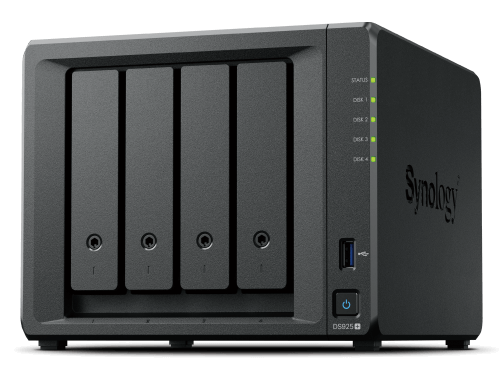
\includegraphics[width=0.8\textwidth]{img/synology.png}
\end{center}
\end{frame}

\begin{frame}
\frametitle{Uma possível solução}

\vspace{0.4cm}
E se construirmos um sistema NAS com um Raspberry Pi 5?
\vspace{0.4cm}

\begin{itemize}
    \item Produto bem mais acessível (com todos os acessórios: $\sim 1400$ reais).
    \item Software customizável e modelado de acordo com o usuário.
    \item Tem um consumo extremamente baixo ($\sim 5$-$7$ W).
\end{itemize}

\end{frame}

\begin{frame}
\frametitle{O projeto Jennie}

\begin{itemize}
    \item Raspberry Pi 5 com HAT para suportar até $5$ HDDs.
    \item Sistema operacional baseado em Linux customizado.
    \item Ventoinhas e cases montadas sob medida.
    \item Sistema de no-break construído do zero para \textit{graceful-shutdown}.
\end{itemize}

\end{frame}

\begin{frame}
\frametitle{Tabela de custos}

\centering
    
    \begin{table}
        \renewcommand{\arraystretch}{1.3}
        \begin{tabular}{lr}
            \toprule
            \textbf{Componentes} & \textbf{Custo (R\$)} \\
            \midrule
            Sistema NAS & 1.283,46 \\
            Sistema No-break & 240,72 \\
            Acessórios & 247,61 \\
            \midrule
            \textbf{Custo Total} & \textbf{1.771,79} \\
            \bottomrule
        \end{tabular}
    \end{table}
    
    \vspace{0.5cm}
    \scriptsize{* Valores não incluem os Discos Rígidos.}

\end{frame}


\section{Hardware}

\begin{frame}
\frametitle{Idealização do projeto}

\begin{center}
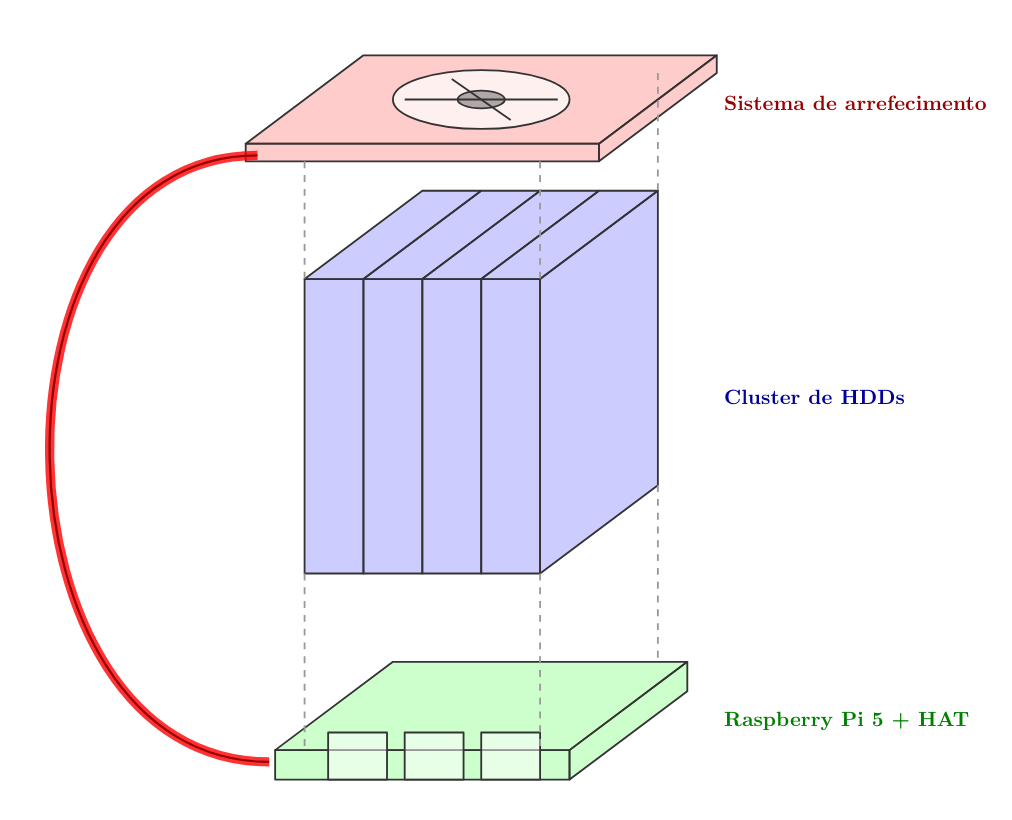
\includegraphics[width=0.8\textwidth]{img/esquema_nas.png}
\end{center}

\end{frame}

\begin{frame}
\frametitle{Componentes de Hardware}

\begin{itemize}
    \item Raspberry Pi 5 com 2 Gb RAM.
    \item HAT para conexão de HDDs.
    \item HAT de ventoinha com controle via GPIO.
    \item No-break construído com BMS e reguladores de tensão.
    \item \textit{Case} impressa em 3D para contenção do sistema.
\end{itemize}

\end{frame}

\begin{frame}
\frametitle{Raspberry Pi 5}

\begin{center}
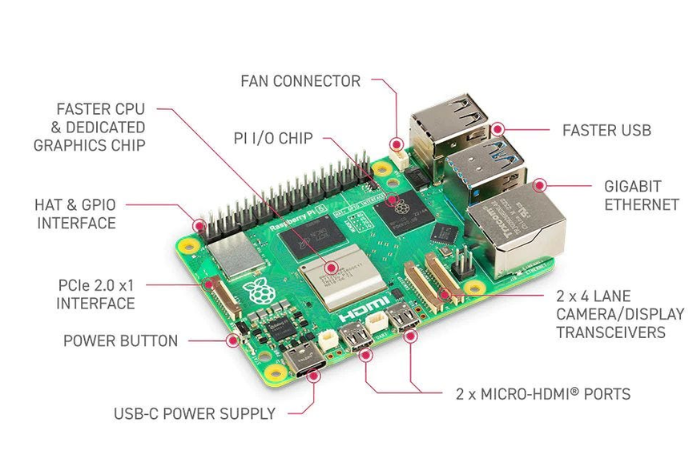
\includegraphics[width=0.85\textwidth]{img/rasp.png}
\end{center}

\end{frame}

\begin{frame}
\frametitle{Radxa Penta SATA HAT}

\begin{center}
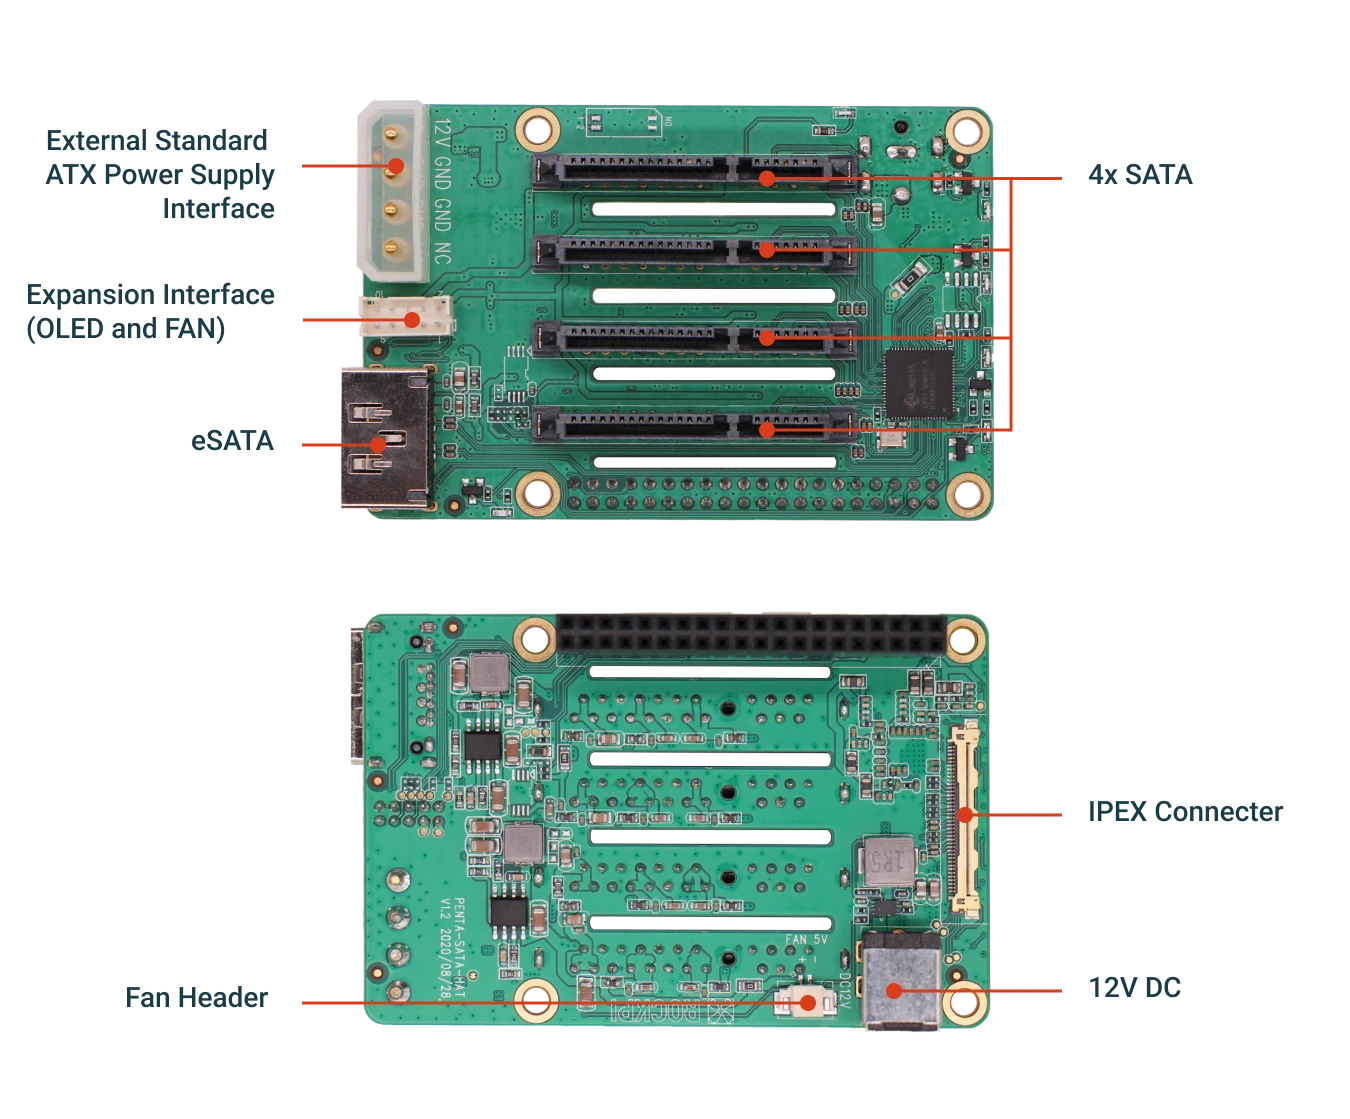
\includegraphics[width=0.85\textwidth]{img/satahat.png}
\end{center}

\end{frame}

\begin{frame}
\frametitle{Radxa SATA HAT Top Board}

\begin{center}
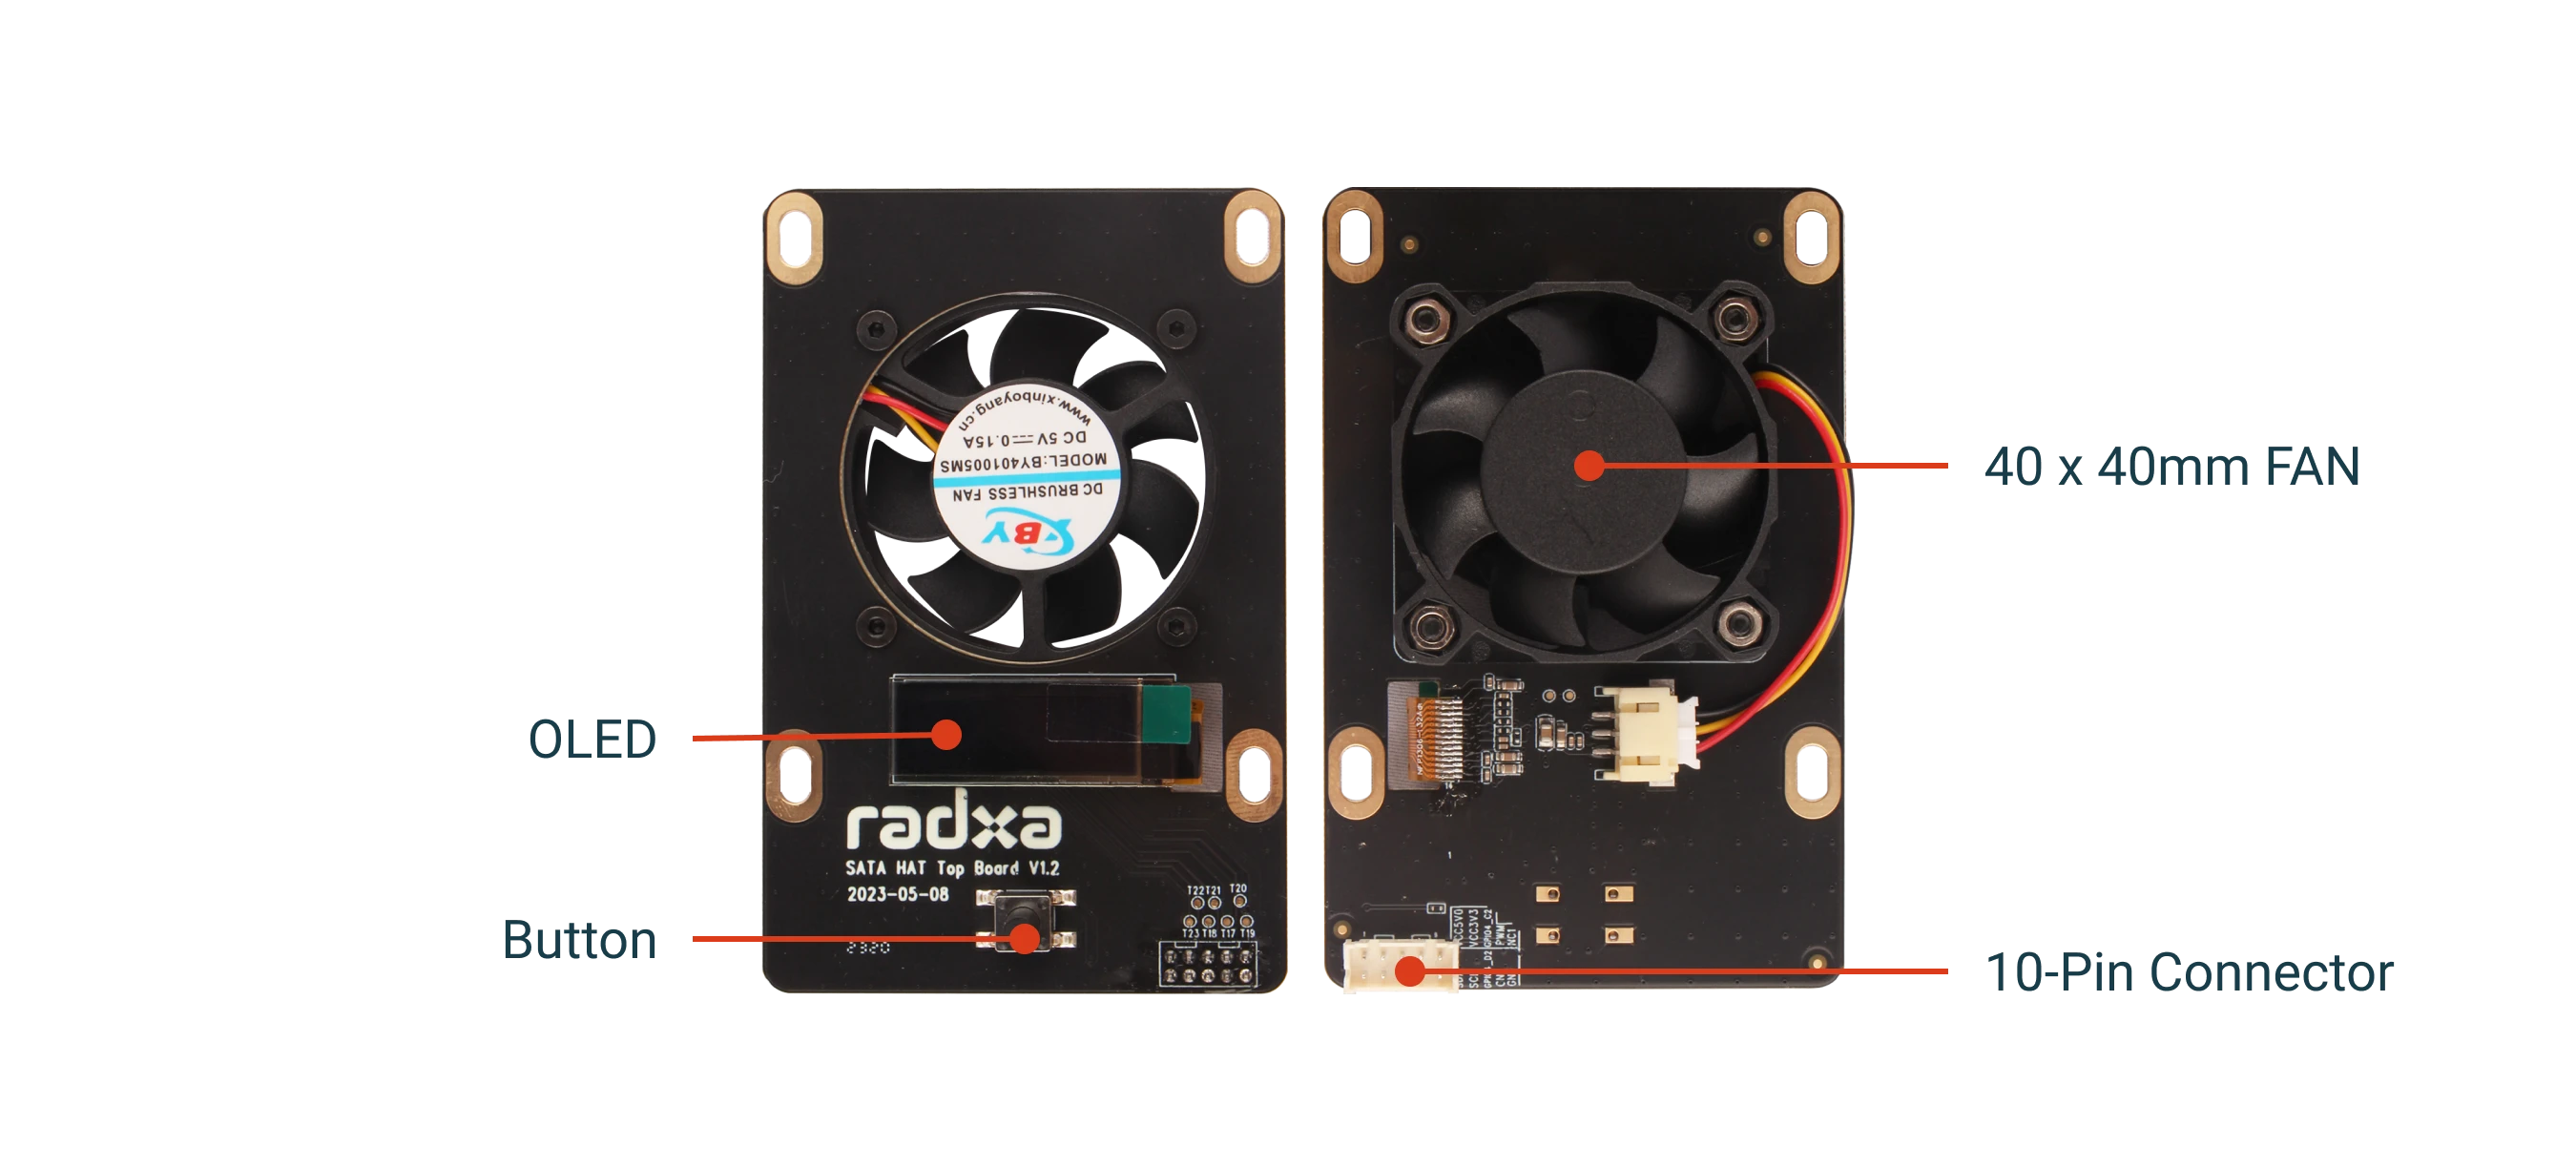
\includegraphics[width=\textwidth]{img/ventoinha.png}
\end{center}

\end{frame}

\begin{frame}
\frametitle{Esquemático do No-Break}

\begin{center}
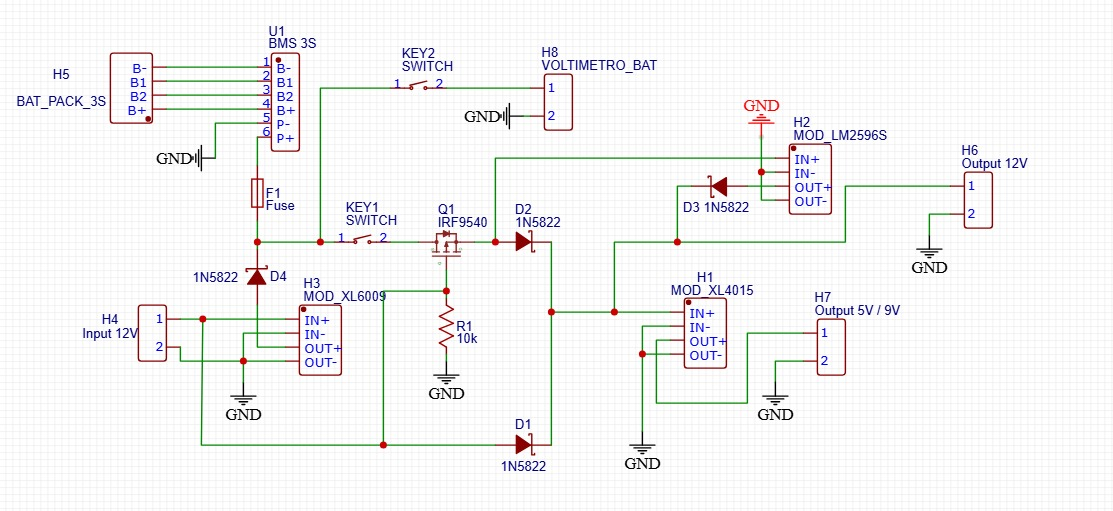
\includegraphics[width=\textwidth]{img/nobreak.png}
\end{center}

\end{frame}

\begin{frame}
\frametitle{Construção do No-Break}

\begin{center}
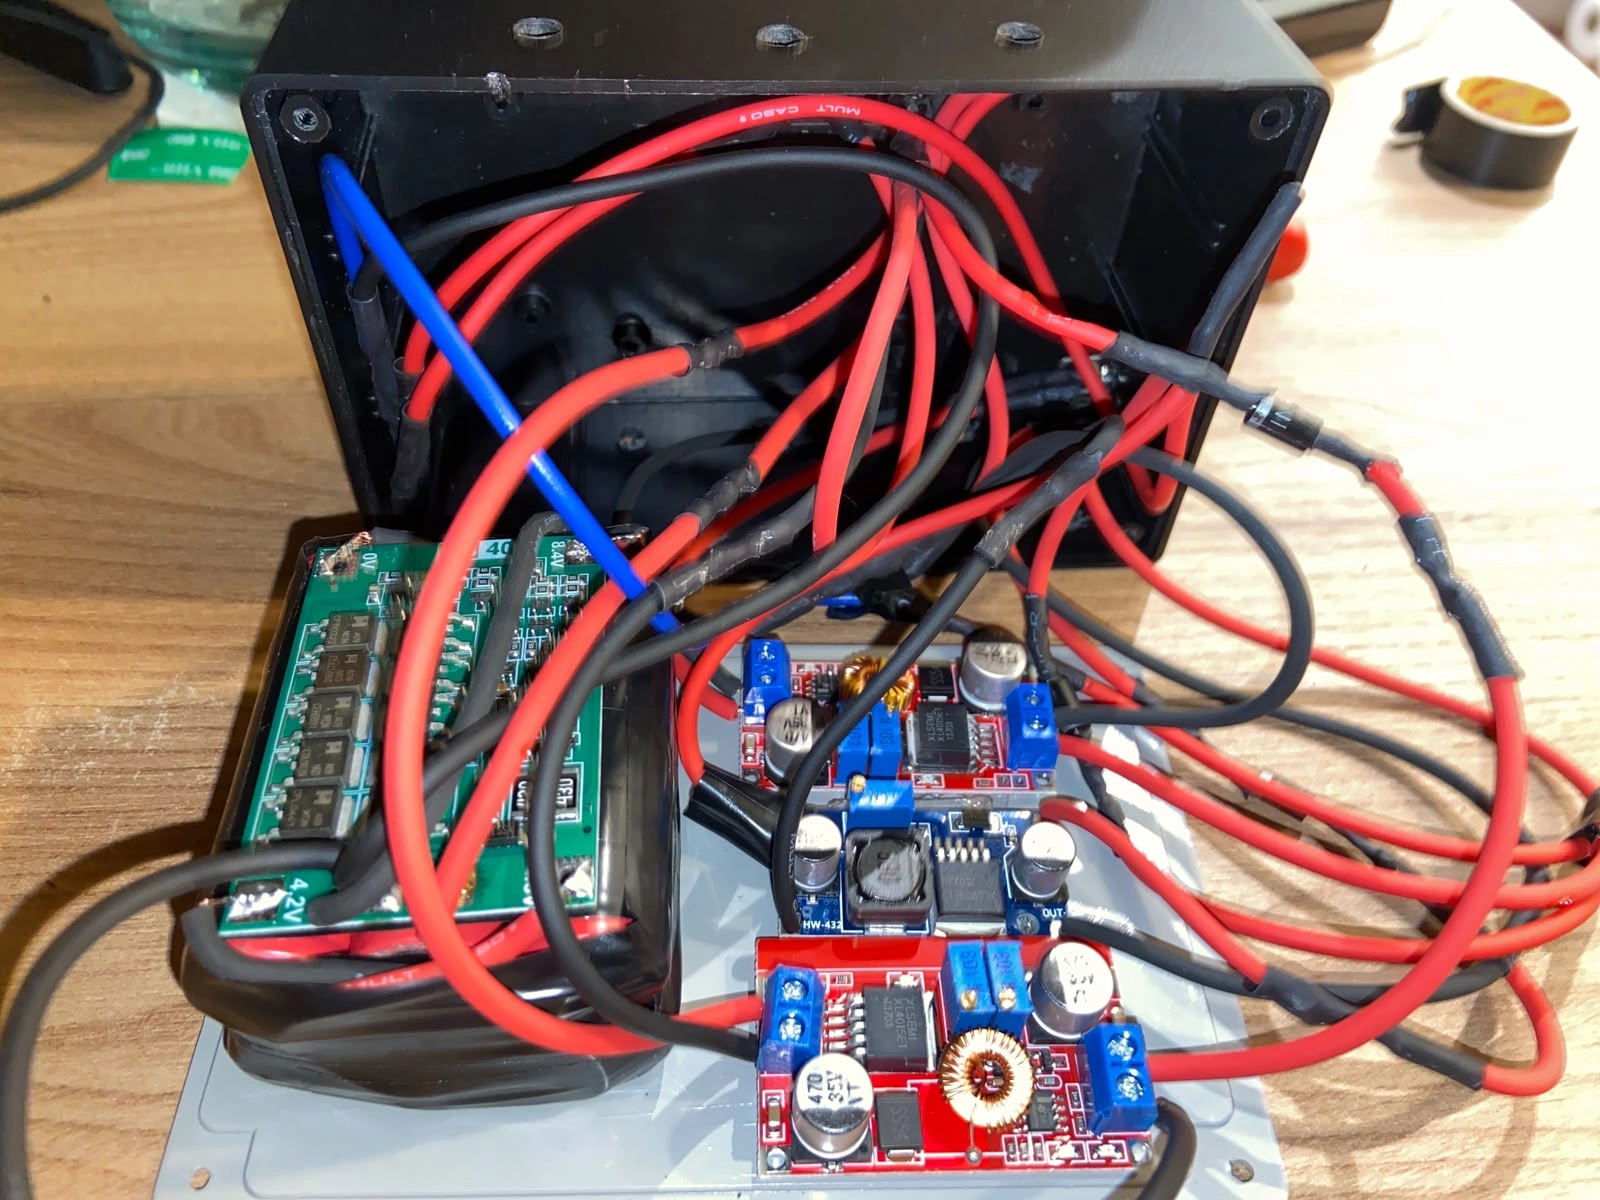
\includegraphics[width=0.9\textwidth]{img/nobreak2.png}
\end{center}

\end{frame}

\begin{frame}
\frametitle{Construção do No-Break}

\begin{center}
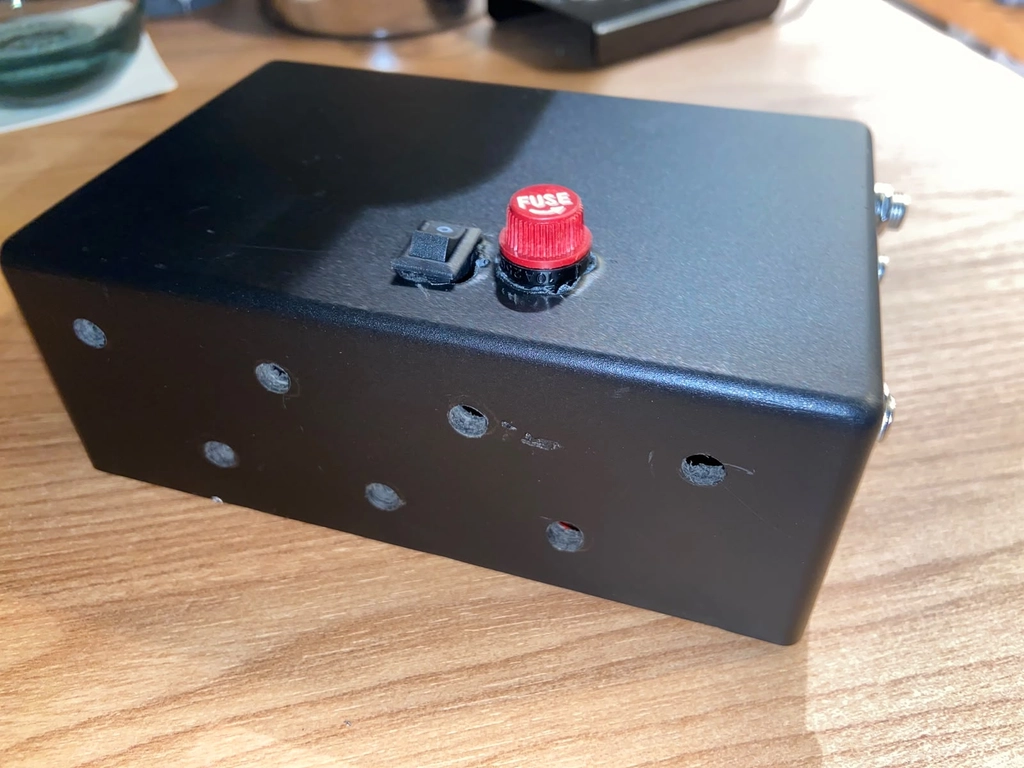
\includegraphics[width=0.9\textwidth]{img/nobreak3.png}
\end{center}

\end{frame}

\begin{frame}
\frametitle{\textit{Case} do sistema}

\begin{center}
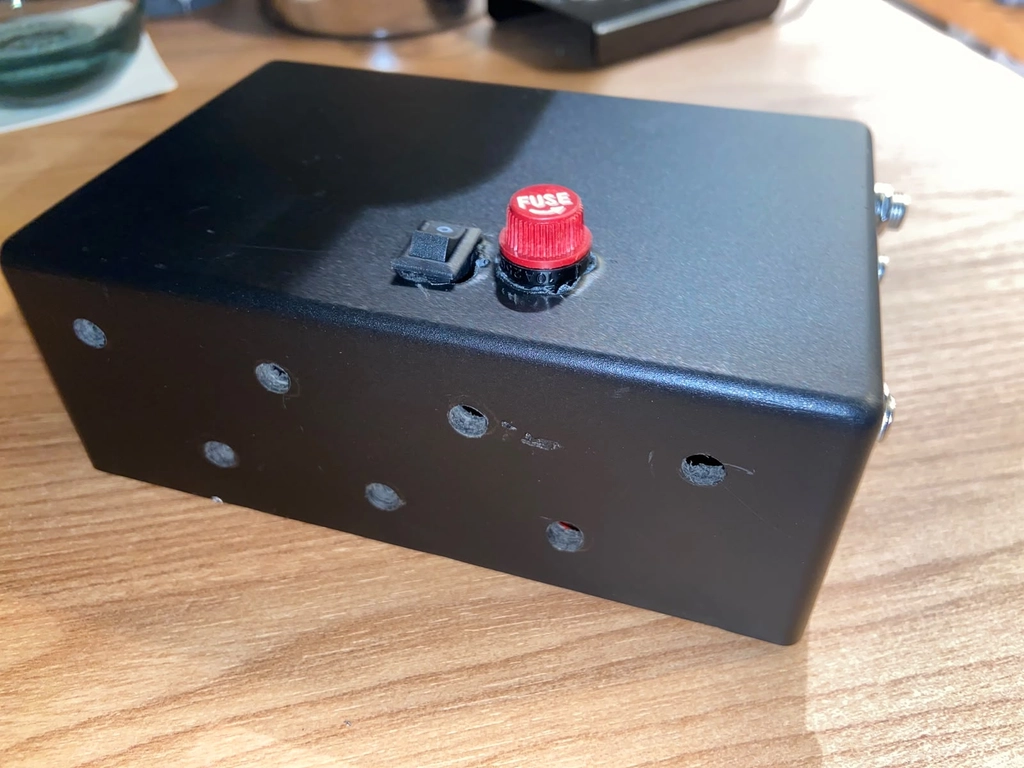
\includegraphics[width=0.9\textwidth]{img/nobreak3.png}
\end{center}

\end{frame}


\section{Software}

\begin{frame}
\frametitle{Proposta do SO}

\begin{columns}[c] 
    
    
    \begin{column}{0.6\textwidth}
        \begin{itemize}
            \item Gentoo Linux!
            \item Distribuição \textit{source-based}.
            \item Configuração e compilação do kernel com \textit{flags} customizadas.
            \item \texttt{Systemd} vs. \texttt{OpenRC}.
        \end{itemize}
    \end{column}
    
    
    \begin{column}{0.35\textwidth}
        \centering
        
\includegraphics[width=\textwidth]{img/gentoo.png}
    \end{column}

\end{columns}
\end{frame}

\begin{frame}
\frametitle{Configuração das USE Flags}

\begin{center}
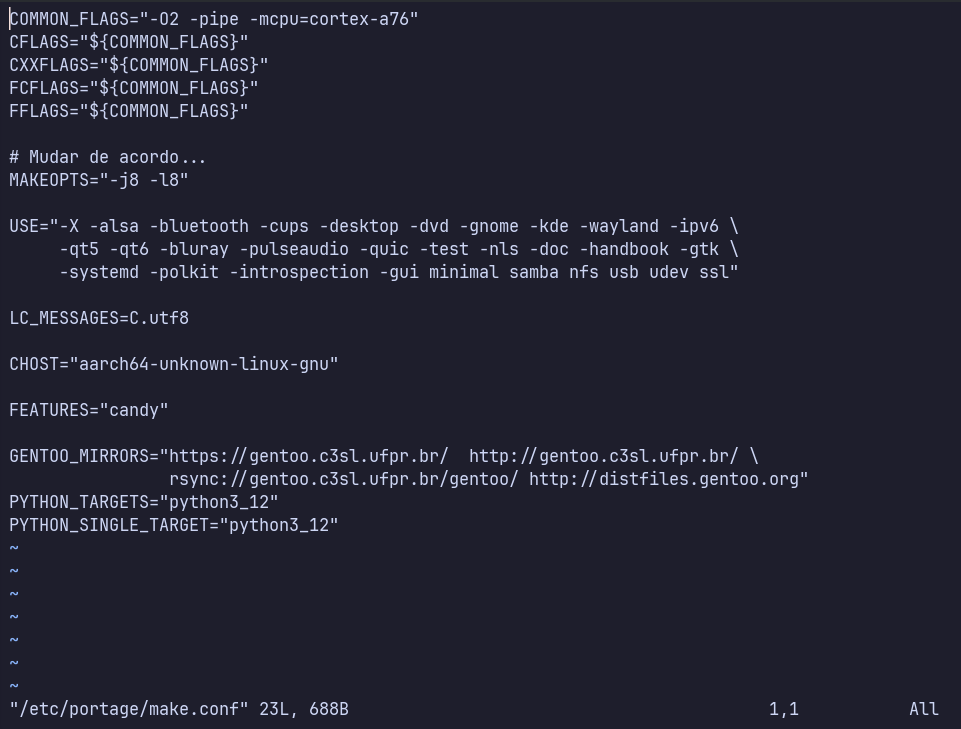
\includegraphics[width=\textwidth]{img/useflags.png}
\end{center}

\end{frame}

\begin{frame}
\frametitle{Algumas configurações do kernel}

\begin{itemize}
    \item Paginação de $16$k.
    \item Quantum de $50$ ms.
    \item Sem suporte a áudio, bluetooth, entre outros.
    \item Instruções assembly otimizadas para ARM Cortex-A76.
\end{itemize}

\end{frame}

\begin{frame}
\frametitle{Interação com o usuário}

\begin{itemize}
    \item Wireguard + SSH.
    \item Interface gráfica.
    \item OLED da ventoinha controlada por scripts em Python.
    \item DuckDNS para IP externo.
    \item Sistema multiuser com \texttt{Podman} para rodar serviços.
\end{itemize}

\end{frame}


\begin{frame}
\frametitle{Interface gráfica}

\begin{center}
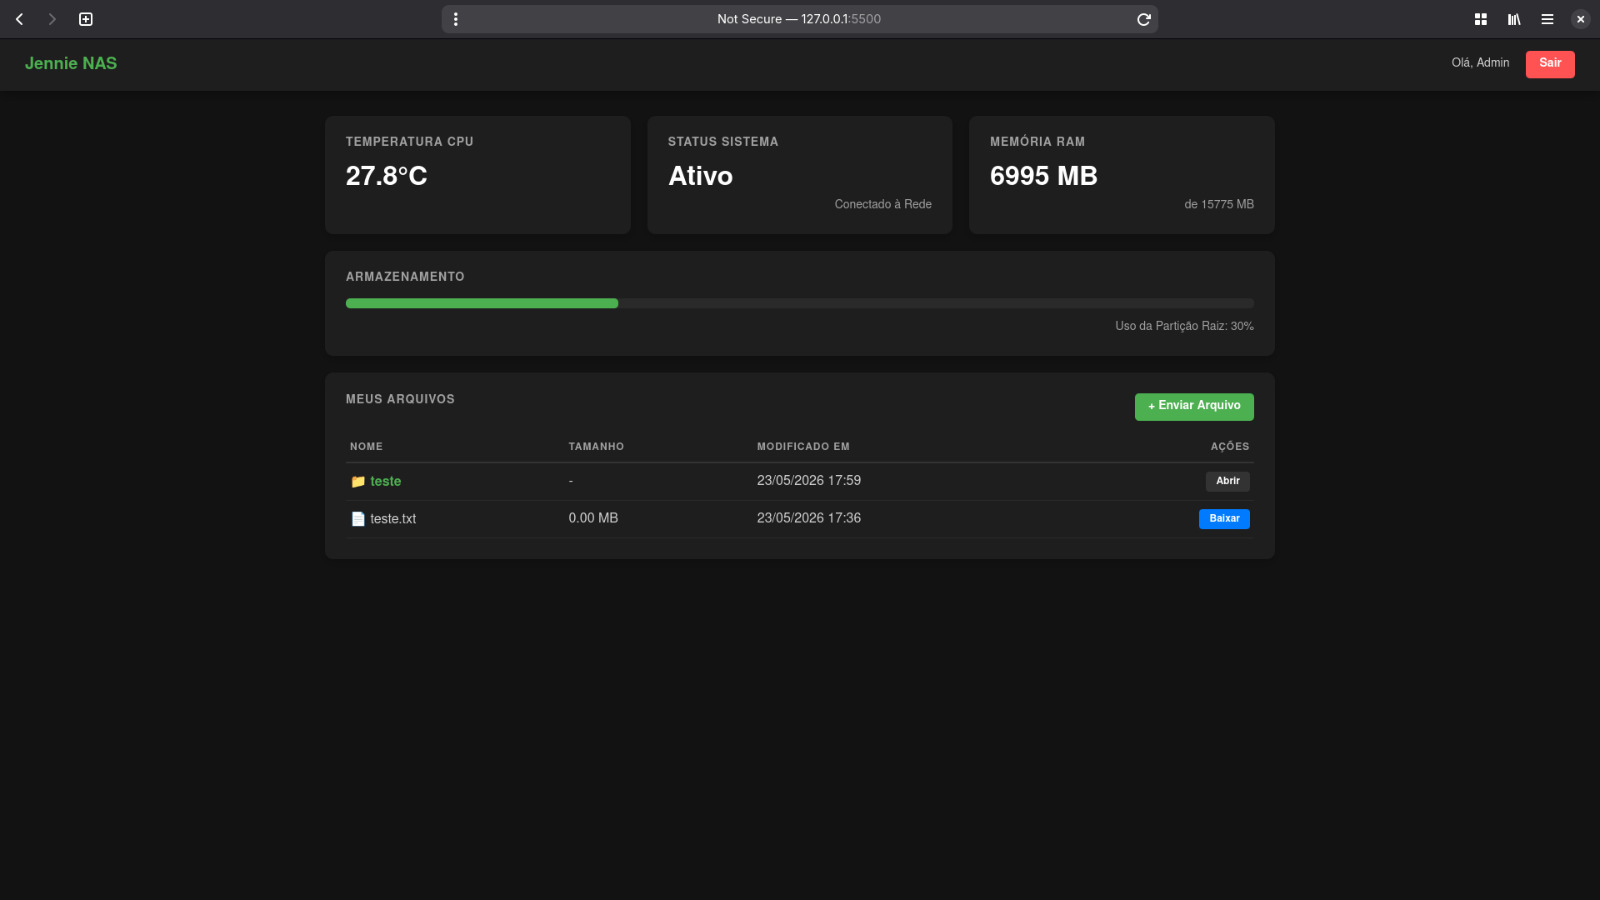
\includegraphics[width=\textwidth]{img/interface.jpg}
\end{center}

\end{frame}


\section{Resultados}



\section{Conclusões}



\end{document}